\documentclass[11pt]{article}
%\usepackage[14pt]{extsizes} % для того чтобы задать нестандартный 14-ый размер шрифта
%\usepackage[utf8]{inputenc}
\usepackage{mathtext}
\usepackage[english, russian]{babel}
\usepackage{amsmath}
\usepackage{amsfonts}
\usepackage{float}
\usepackage[margin=0.8in]{geometry}
\usepackage{multirow}
\usepackage{graphicx}
\usepackage[utf8x]{inputenc} % указать кодировку русского текста
\usepackage{fancyhdr}
\usepackage{indentfirst} % отступ в первой строке абзаца
\usepackage{wrapfig}
\usepackage{placeins}
\usepackage{wrapfig}
\usepackage{caption}
\usepackage{amssymb}
\usepackage{mathtools}
\usepackage[thinc]{esdiff}
%\usepackage{ upgreek }

\pagestyle{fancy}
\begin{document}
\begin{titlepage}
\begin{center}
%\vspace*{1cm}
\large{\small ФЕДЕРАЛЬНОЕ ГОСУДАРСТВЕННОЕ АВТОНОМНОЕ ОБРАЗОВАТЕЛЬНОЕ\\ УЧРЕЖДЕНИЕ ВЫСШЕГО ОБРАЗОВАНИЯ\\ МОСКОВСКИЙ ФИЗИКО-ТЕХНИЧЕСКИЙ ИНСТИТУТ\\ (НАЦИОНАЛЬНЫЙ ИССЛЕДОВАТЕЛЬСКИЙ УНИВЕРСИТЕТ)\\ ФИЗТЕХ-ШКОЛА РАДИОТЕХНИКИ И КОМПЬЮТЕРНЫХ ТЕХНОЛОГИЙ}
\vfill
\line(1,0){430}\\[1mm]
\huge{Лабораторная работа 2.2.5}\\
\huge\textbf{Определение вязкости жидкости по скорости истечения через капилляр}\\
\line(1,0){430}\\[1mm]
\vfill
\begin{flushright}
\normalsize{Устюжанина Мария}\\
\normalsize{\textbf{Группа Б01-107}}\\
\end{flushright}
\end{center}
\end{titlepage}
\fancyhead[L] {Работа 2.2.5}


\par \textbf{Цель работы:} 1) определение вязкости воды по измерению объема жидкости, протекшей через капилляр; 2) определение вязкости других жидкостей путем сравнения скорости их перетекания со скоростью перетекания воды.
\par \textbf{В работе используются:} сосуд Мариотта; капиллярная трубка; мензурка; секундомер; стакан; микроскоп на стойке; вискозиметр Оствальда.

\section{Введение.}

В данной работе исследуется определение вязкости жидкости по скорости истечения ее через капилляр. Работа будет состоять из 2х частей: изменрения вязкости воды с помощью сосуда Мариотта и измерения вязкости водного раствора глицерина вискозиметром Оствальда. Схемы установок:

\begin{figure}[H]
\centering
\captionsetup{justification=centering}
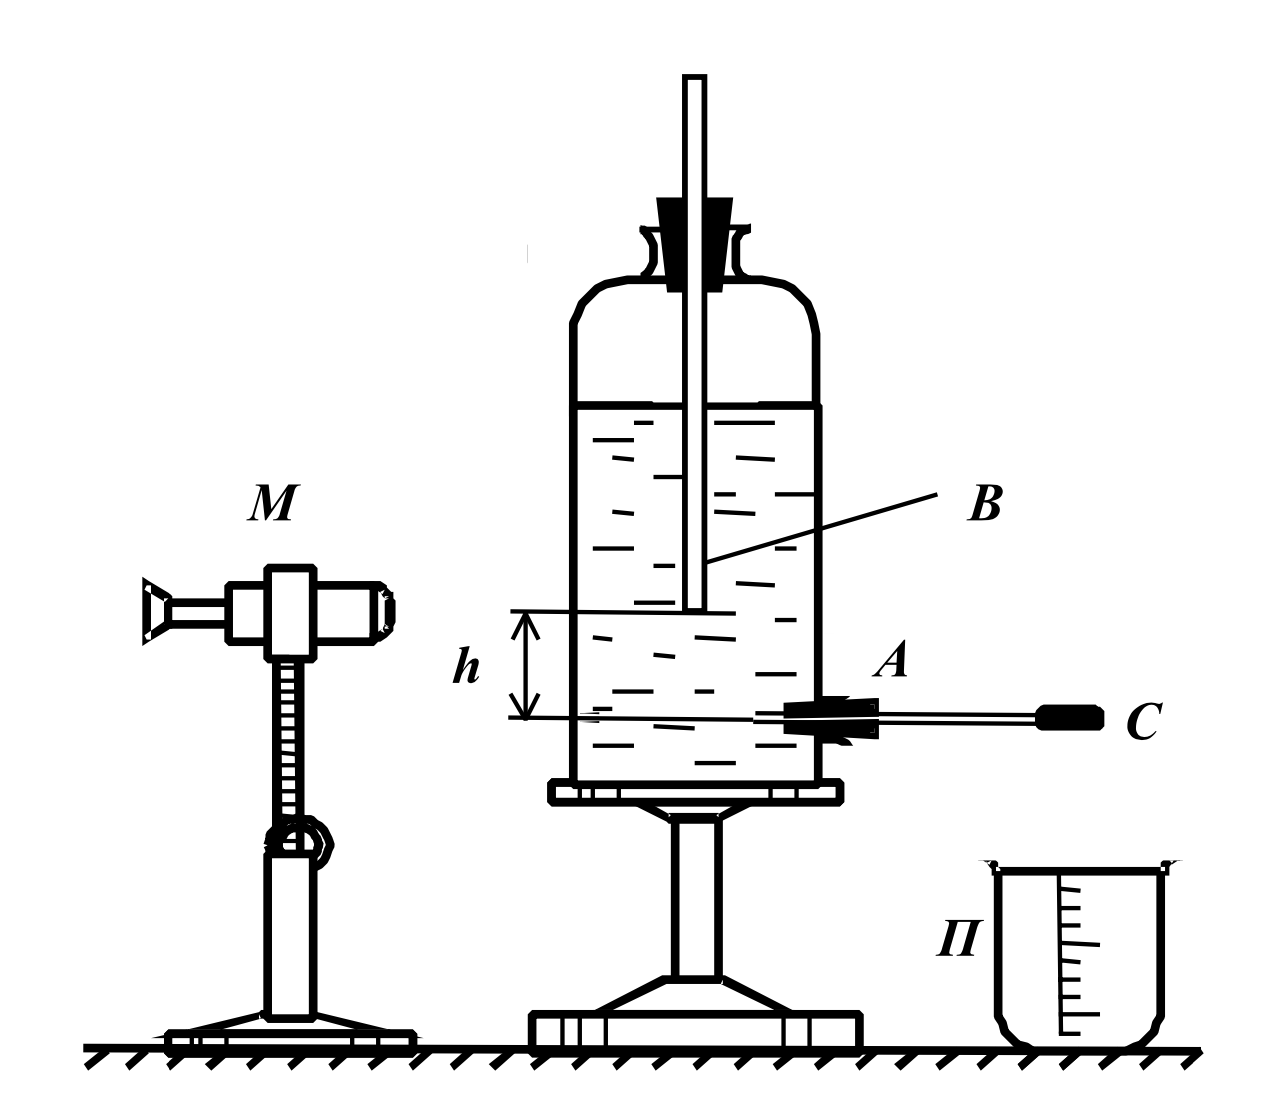
\includegraphics[width=0.5\textwidth]{Pic1.png}
\caption{Схема установки для определения вязкости воды}
\end{figure}

\begin{figure}[H]
\centering
\captionsetup{justification=centering}
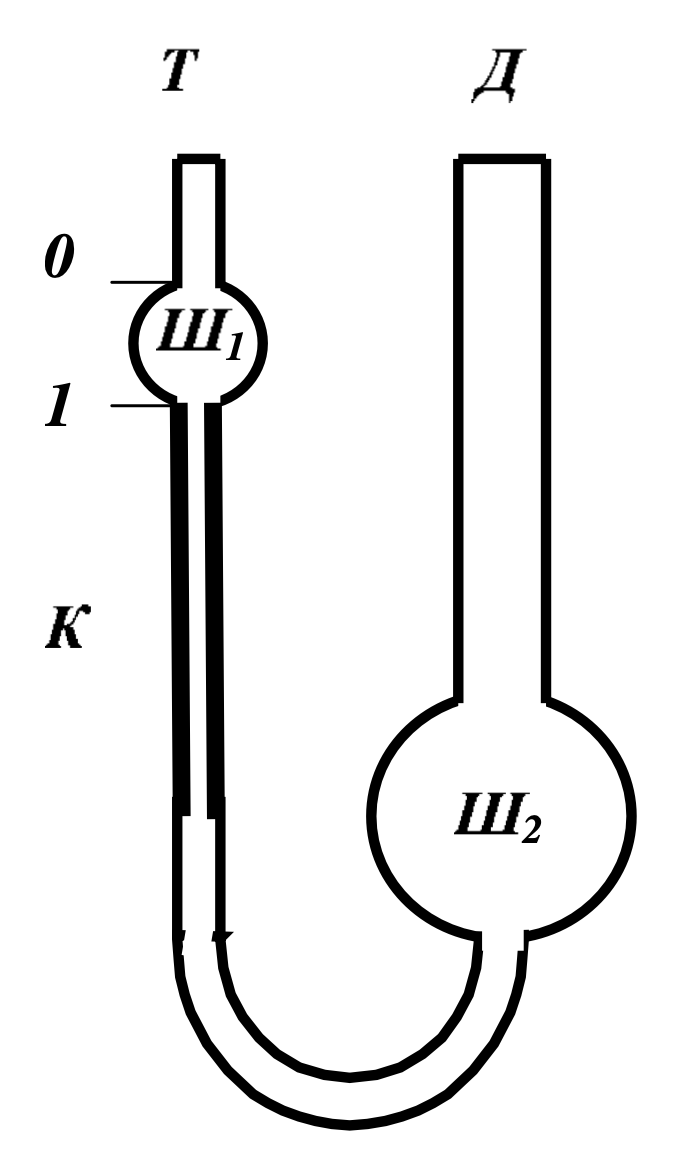
\includegraphics[width=0.25\textwidth]{Pic2.png}
\caption{Вискозиметр Оствальда. Вискозиметр Оствальда (рис. 3) представляет собой U-образную стеклянную трубку. Одно колено прибора в верхней части имеет расширение — шарик Ш1 с метками «0» и «1» — и капилляр К. Другое колено представляет собой широкую трубку Д с резервуаром — шариком Ш2.}
\end{figure}


\section{Обработка данных:}
\subsection{Измерение вязкости воды}
\begin{enumerate}
    \item Измерим параметры капиляра:

    \begin{table}[H]
    \centering
    \begin{tabular}{l}
    Длина капилярa = 131 мм \\
    Диаметр капилярa = 9 мм
    \end{tabular}
    \end{table}


    \item Дождавшись установившегося режима вытекания воды через капиляр(появились первые пузырьки на нижнем конце трубки В), мы провели 2 измерения времени, за которое мензурка заполняется на 25 мл. $t_1 = 185c, t_2 = 180c (h = 85мм)$. Такие данные убеждают нас в том, что скорость истечения не зависит от количества воды в сосуде, а определяется глубиной погружения трубки В.

    \item Приступим к основной серии измерений. Мы будем менять глубину погружения трубки В и измерять время, за которое через капилляр вытечет 20 мл воды.

    \begin{table}[H]
    \centering
    \caption{\textbf{Результаты измерений}}
    \begin{tabular}{|l|l|l|l|l|l|}
    \hline
    \textbf{h,  мм} & 29  & 38  & 44  & 57  & 62  \\ \hline
    \textbf{t, c}   & 576 & 383 & 327 & 248 & 213 \\ \hline
    \end{tabular}
    \end{table}

    \item Будем вычислять раcход воды Q, оценивать число Рейнольдса Re (взяв вязкость воды $\eta \approx 0,01 П$) и длину участка копиляра, на котором устанавливается ламинарное течение, по следующим формулам: 

    \[ Q = \frac{V}{t}\]
    \[ Re = \frac{ Q R \rho }{S \eta}\]
    \[ a \approx 0,2 R \cdot Re \]


    \begin{table}[H]
    \centering
    \caption{\textbf{Полученные данные}}
    \begin{tabular}{|l|r|r|r|r|r|}
    \hline
    \textbf{h, мм}    & 29   & 38   & 44   & 57   & 62   \\ \hline
    \textbf{Q, мкл/с} & 35   & 52   & 61   & 81   & 94   \\ \hline
    \textbf{Re}       & 2,5  & 3,69 & 4,3  & 5,73 & 6,65 \\ \hline
    \textbf{a, мм}    & 2,25 & 3,32 & 3,87 & 5,16 & 5,98 \\ \hline
        \end{tabular}
    \end{table}

    По полученным данным построим график:

    \begin{figure}[H]
    \centering
    \captionsetup{justification=centering}
    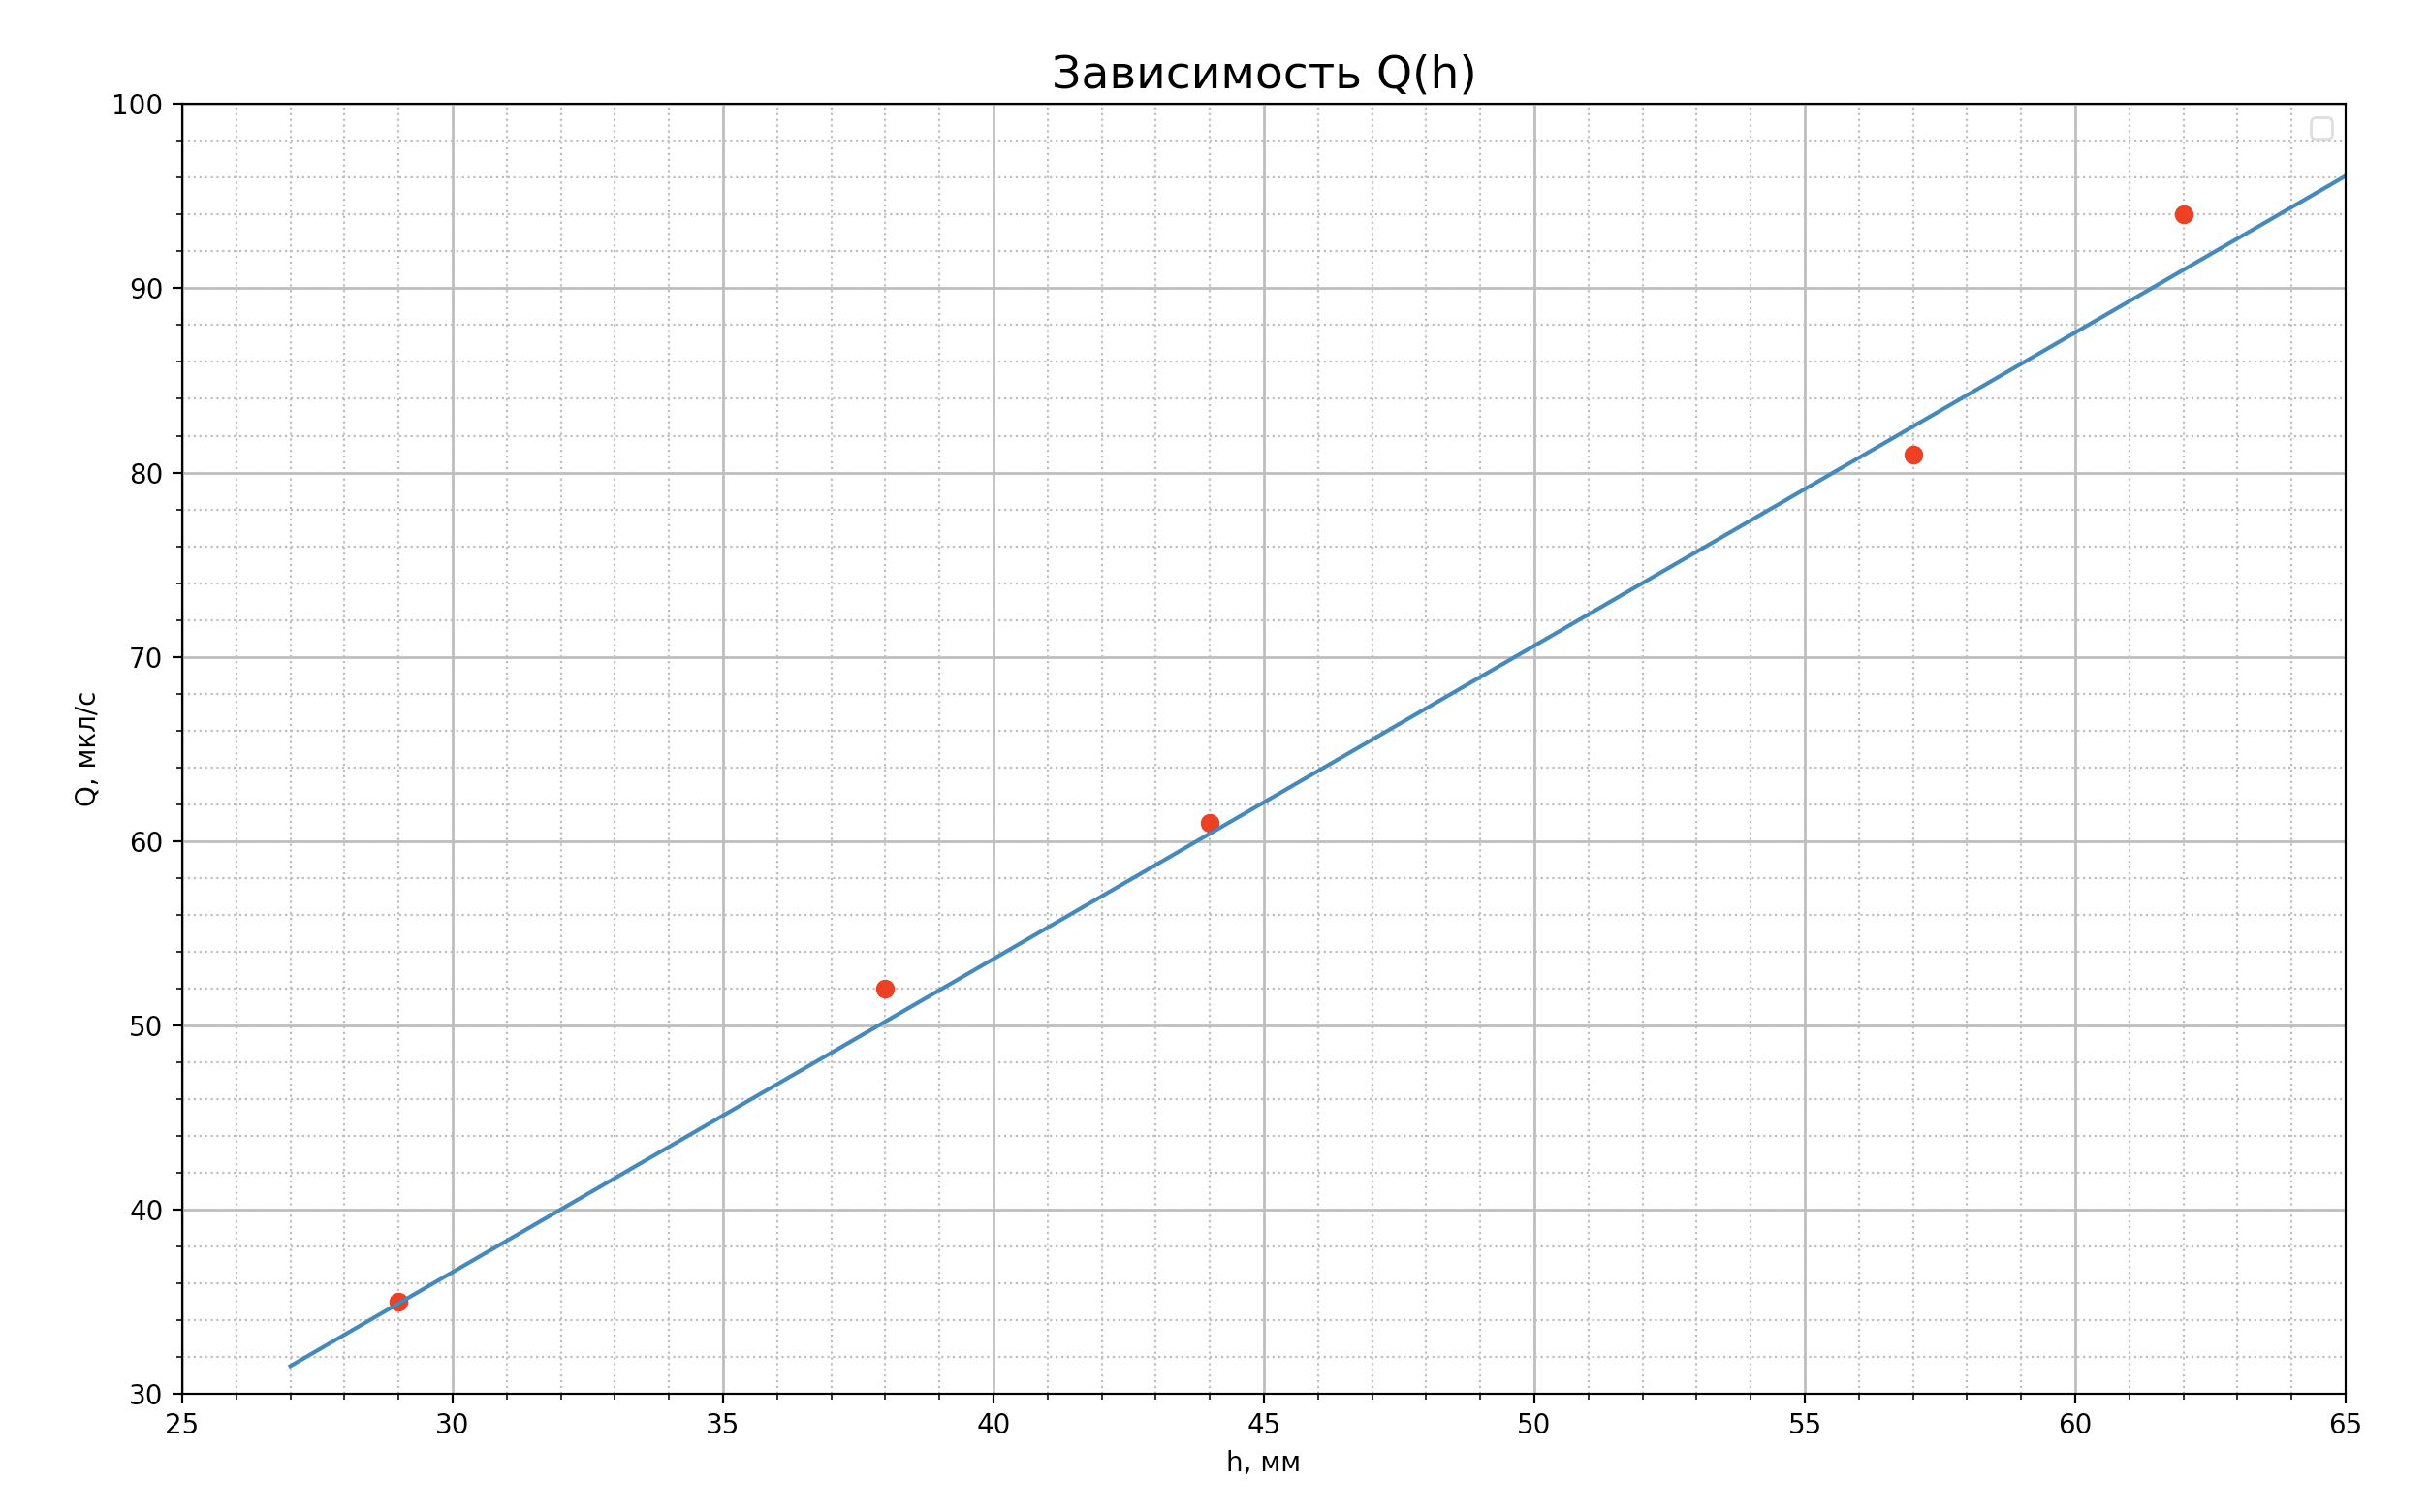
\includegraphics[width=\textwidth]{Graf1}
    \caption{}
    \end{figure}

    Получена линейная зависимость $y = (1,7\pm 0,1)x - (14\pm1)$. По углу наклона графика определим вязкость воды:
    \[ \eta = \frac{\pi R^4 \rho g}{8lQ'(h)} \approx (7,2\cdot 10^{-3})П\]

    Табличное значение: $0.011 П$
\subsection{Измерение вязкости раствора глицерина вискозиметром Освальда}

    Измерим время протекания жидкостей между отметками вискозиметра.

    \begin{table}[H]
    \centering
    \caption {\textbf{Результаты измерений}}
    \begin{tabular}{|l|r|r|r|r|r|r|r|}
    \hline
    \textbf{Номер опыта}         & 1     & 2     & 3     & 4     & 5     & \multicolumn{1}{l|}{Ср. знач.} & \multicolumn{1}{l|}{Погрешность} \\ \hline
    \textbf{t воды, с}           & 5,91  & 5,87  & 5,84  & 5,89  & 6,09  & 5,92                           & 0,04                             \\ \hline
    \textbf{t глицерина 10\%, с} & 8,32  & 8,36  & 8,33  & 8,68  & 8,86  & 8,51                           & 0,3                              \\ \hline
    \textbf{t глицерина 20\%, с} & 10,72 & 11,35 & 10,65 & 10,75 & 11,17 & 10,94                          & 0,4                              \\ \hline
    \textbf{t глицерина 30\%, с} & 15,15 & 15,18 & 15,49 & 15,19 & 15,18 & 15,2                           & 0,1                              \\ \hline
    \end{tabular}
    \end{table}

    Вязкость растворов глицерина получем с помощью формулы:
    \[ \eta_x = \eta_0 \frac{\rho_x \cdot t_x}{\rho_0 \cdot t_0}\]

    Полученные значения: 

    \begin{table}[H]
    \centering
    \begin{tabular}{|r|r|}
    \hline
    \multicolumn{1}{|l|}{\textbf{Глицерин, \%}} & \multicolumn{1}{l|}{\textbf{$\eta$, $П\cdot c$}} \\ \hline
    10                                          & 1,1                                 \\ \hline
    20                                          & 1,4                                 \\ \hline
    30                                          & 2                                   \\ \hline
    \end{tabular}
    \end{table}

    Значения достаточно точно совпадают с табличными: 

    \begin{table}[H]
    \centering
    \begin{tabular}{|r|r|}
    \hline
    \multicolumn{1}{|l|}{\textbf{Глицерин, \%}} & \multicolumn{1}{l|}{\textbf{$\eta$, $П\cdot c$}} \\ \hline
    10                                          & 1,0                                \\ \hline
    20                                          & 1,31                                 \\ \hline
    30                                          & 2,5                                  \\ \hline
    \end{tabular}
    \end{table}


\end{enumerate}



\section{Вывод} 

    В ходе лабораторной работы нам удалось измерить вязкость жидкдостей двумя разными способами:


    1) Определили вязкость воды через скорость истечения жидкости через капиляр из сосуда Мариотта по формуле Пуазейля. Полученное значение получилось довольно близким к табличному.


    2) Далее мы наблюдали за скоростью протекания жидости через вискозиметр Оствальда и через зависимость вязкости от времени протекания и плотности получали плотность растворов глицерина. Полученные данные хорошо совпадали с табличными.



\end{document}